

\chapter{Sprint 0}
\label{Sprint0}
\lhead{Chapter 6. \emph{Sprint 0}}

This chapter is meant to cover our first sprint, sprint 0. 


\section{Sprint goal(s)}

Our first sprint was focused on project planning and preliminary studies.
The goal of this sprint was to achieve a sufficient understanding of the problem scope in order
perform studies on existing technologies that we could use and similar existing solutions.

\section{Sprint breakdown}

\begin{figure}[H]
\centering
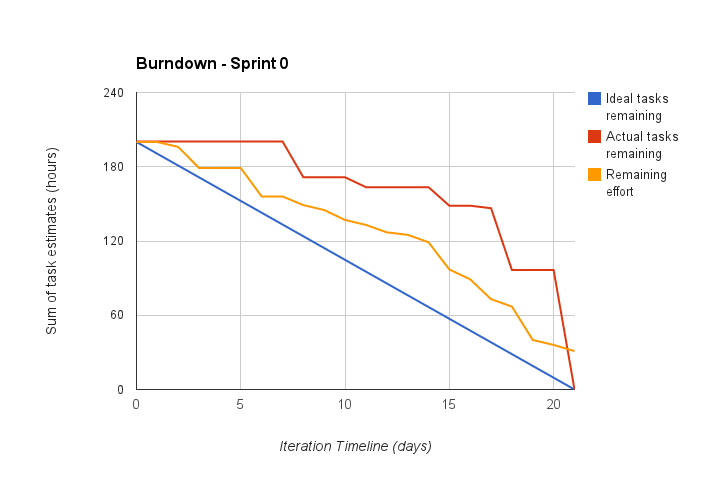
\includegraphics[scale=0.50]{../Figures/burndownSprint0.png}
\caption{Burndown chart Sprint 0}
\label{figure:burndownsprint0}
\end{figure}


\subsection{Duration}
This project started on wednesday 21.08.2013 which was the first day of the project and the day we meet the group, the supervisor, the client and got acquainted with the project. We decided early on to use the /ref{Scrum} methodology and to have short sprints so we could focus on some areas at a time. We landed on a total of 6 sprints that each lasted two weeks for a totalt of 12 weeks. Even though we didn't agree on this method before monday the 26th of august we have added the first few days to the first sprint so they also belong in a sprint for tracking the work. Hence the first sprint also includes the first few days of the project making it a total of 13 weeks. 
The duration of the sprint was the following:
\begin{itemize}
\item Sprint start: August, 21th
\item Sprint end: September, 8th
\end{itemize}

\subsection{Planning} 

\subsection{Backlog}

\begin{description}
\item[test]
\end{description}


include sprint backlog and burndown chart
\subsection{Results and feedback}
from customer, from supervisor
\subsection{Evaluation}
our thoughts about this sprint
